\subsection{Hopf bifurcation on 1-d mesa patterns}
\label{sec:hopf}

The eigenvalues of 1-d mesa patterns are given by \eqref{eqn:lam_pm}, when taking $m=0$,
% 
\begin{equation}
\begin{split}
\label{eqn:lam_pm_m}
  \lA_+ &= \frac{\Ep^2}{\vA}\left[\oM_+ + \left(1-\frac{L}{l} \right)\frac{l^2}{L^2}L\right],\\
  \lA_- &= \frac{\Ep^2}{\vA}\left[\oM_- + \left(1-\frac{L}{l} \right)\frac{l^2}{L^2}L\right],
\end{split}
\end{equation}
% 
where
%
\[
  \begin{split}
    \oM_+ &= \frac{1}{d-e} = [\sI_-\tanh[\sI_-(L-l)]+\sI_+\tanh(l\sI_+)]^{-1},\\
	\oM_- &= \frac{1}{d+e} = [\sI_-\tanh[\sI_-(L-l)]+\sI_+\coth(l\sI_+)]^{-1},\\
  \end{split}
\]
% 
with 
% 
\begin{equation}
\label{eqn:sig_va}
  \sI_{\pm} = \sqrt{\frac{\Ep}{\DD}(\kA_{\pm}+\tau\lA)},\qquad \vA = -\frac{\DD}{g_-}\kA_0\frac{l}{L}.
\end{equation}
% 

\begin{remark}
  There are several distinguished limits in $\tau$ that are relevant.
\end{remark}

Case I: The natural distinguished limit is when $\lA_{\pm} = O(\Ep^2)$. In this limit we need both $\oM_+$ and $\oM_-$ to satisfy $\oM_{\pm}=O(1)$, and thus we require that $\sI_{\pm} = O(1)$  (we showed earlier that $\oM_+$ and $\oM_-$ have different limits as $\sI_{\pm}\rightarrow0$). 

To satisfy this condition we require that $\frac{\Ep\tau\lA}{\DD}=O(1)$ in order to have $\sI_{\pm}=O(1)$. Given that $\lA=O(\Ep^2)$, this means that $\tau=O(\Ep^{-3})$.

The equations can be simplified by eliminating some constants via a suitable change of variables. Let $\tau_0$ and $\La$ be defined as 
% 
\[
  \lA=-\frac{\Ep^2}{\vA}\La,\qquad \tau = -\frac{1}{\Ep^3}\vA\DD\tau_0.
\]
% 

From \eqref{eqn:sig_va} we obtain
% 
\[
  \sI_{\pm} = \sqrt{\tau_0\La} + O(\Ep),
\]
% 
and the equations in \eqref{eqn:lam_pm_m} become
% 
\[
\begin{split}
  \La = -\frac{1}{\sqrt{\tau_0\La}\left[\tanh(\sqrt{\tau_0\La}(L-l)) + \tanh(\sqrt{\tau_0\La}l) \right]} - \left(1-\frac{L}{l}\right)\frac{l^2}{L^2}L ,\\
  \La = -\frac{1}{\sqrt{\tau_0\La}\left[\tanh(\sqrt{\tau_0\La}(L-l)) + \coth(\sqrt{\tau_0\La}l) \right]} - \left(1-\frac{L}{l}\right)\frac{l^2}{L^2}L ,
\end{split}
\]
% 
for the zigzag and breather eigenvalues, respectively.

In order to find the Hopf bifurcation values, we let $\La = i\dE/\tau_0$, and for the zigzag case we get
% 
\[
\begin{split}
  F_+ = \frac{i\dE}{\tau_0} + \frac{1}{\sqrt{i\dE}\left[\tanh(\sqrt{i\dE}(L-l)) + \tanh(\sqrt{i\dE}l) \right]} + \left(1-\frac{L}{l}\right)\frac{l^2}{L^2}L = 0.
\end{split}
\]
% 

We must now find values for $\dE$ and $\tau$ such that
% 
\[
  F_+ = \text{Re}[F_+] + i\text{Im}[F_+] = 0,
\]
% 
hence we require both $\text{Re}[F_+]=0$ and $\text{Im}[F_+]=0$.

We have then that the Hopf bifurcation values in \eqref{eqn:lam_pm_m} are the roots of
% 
\begin{subequations}
\label{eqn:hopf1}
\begin{align}
\label{eqn:hopf1a}
  &\text{Re}\left[\frac{1}{\sqrt{i\dE}\left[\tanh(\sqrt{i\dE}(L-l)) + \tanh(\sqrt{i\dE}l) \right]}\right] + \left(1-\frac{L}{l}\right)\frac{l^2}{L^2}L = 0,\\
\label{eqn:hopf1b}
  &\text{Im}\left[\frac{1}{\sqrt{i\dE}\left[\tanh(\sqrt{i\dE}(L-l)) + \tanh(\sqrt{i\dE}l) \right]}\right] + \frac{\dE}{\tau_0} = 0.
\end{align}
\end{subequations}
% 

This setup decouples the system in terms of finding $\dE$ and $\tau_0$. To find both values one must start by solving \eqref{eqn:hopf1a} in terms of $\dE$, and then substitute the values into \eqref{eqn:hopf1b} in order to find $\tau_0$
% 
\[
  \tau_0 = -\frac{\dE}{\text{Im}\left[\frac{1}{\sqrt{i\dE}\left[\tanh(\sqrt{i\dE}(L-l)) + \tanh(\sqrt{i\dE}l) \right]}\right]}
\]
% 
\begin{figure}[htb]
\begin{center}
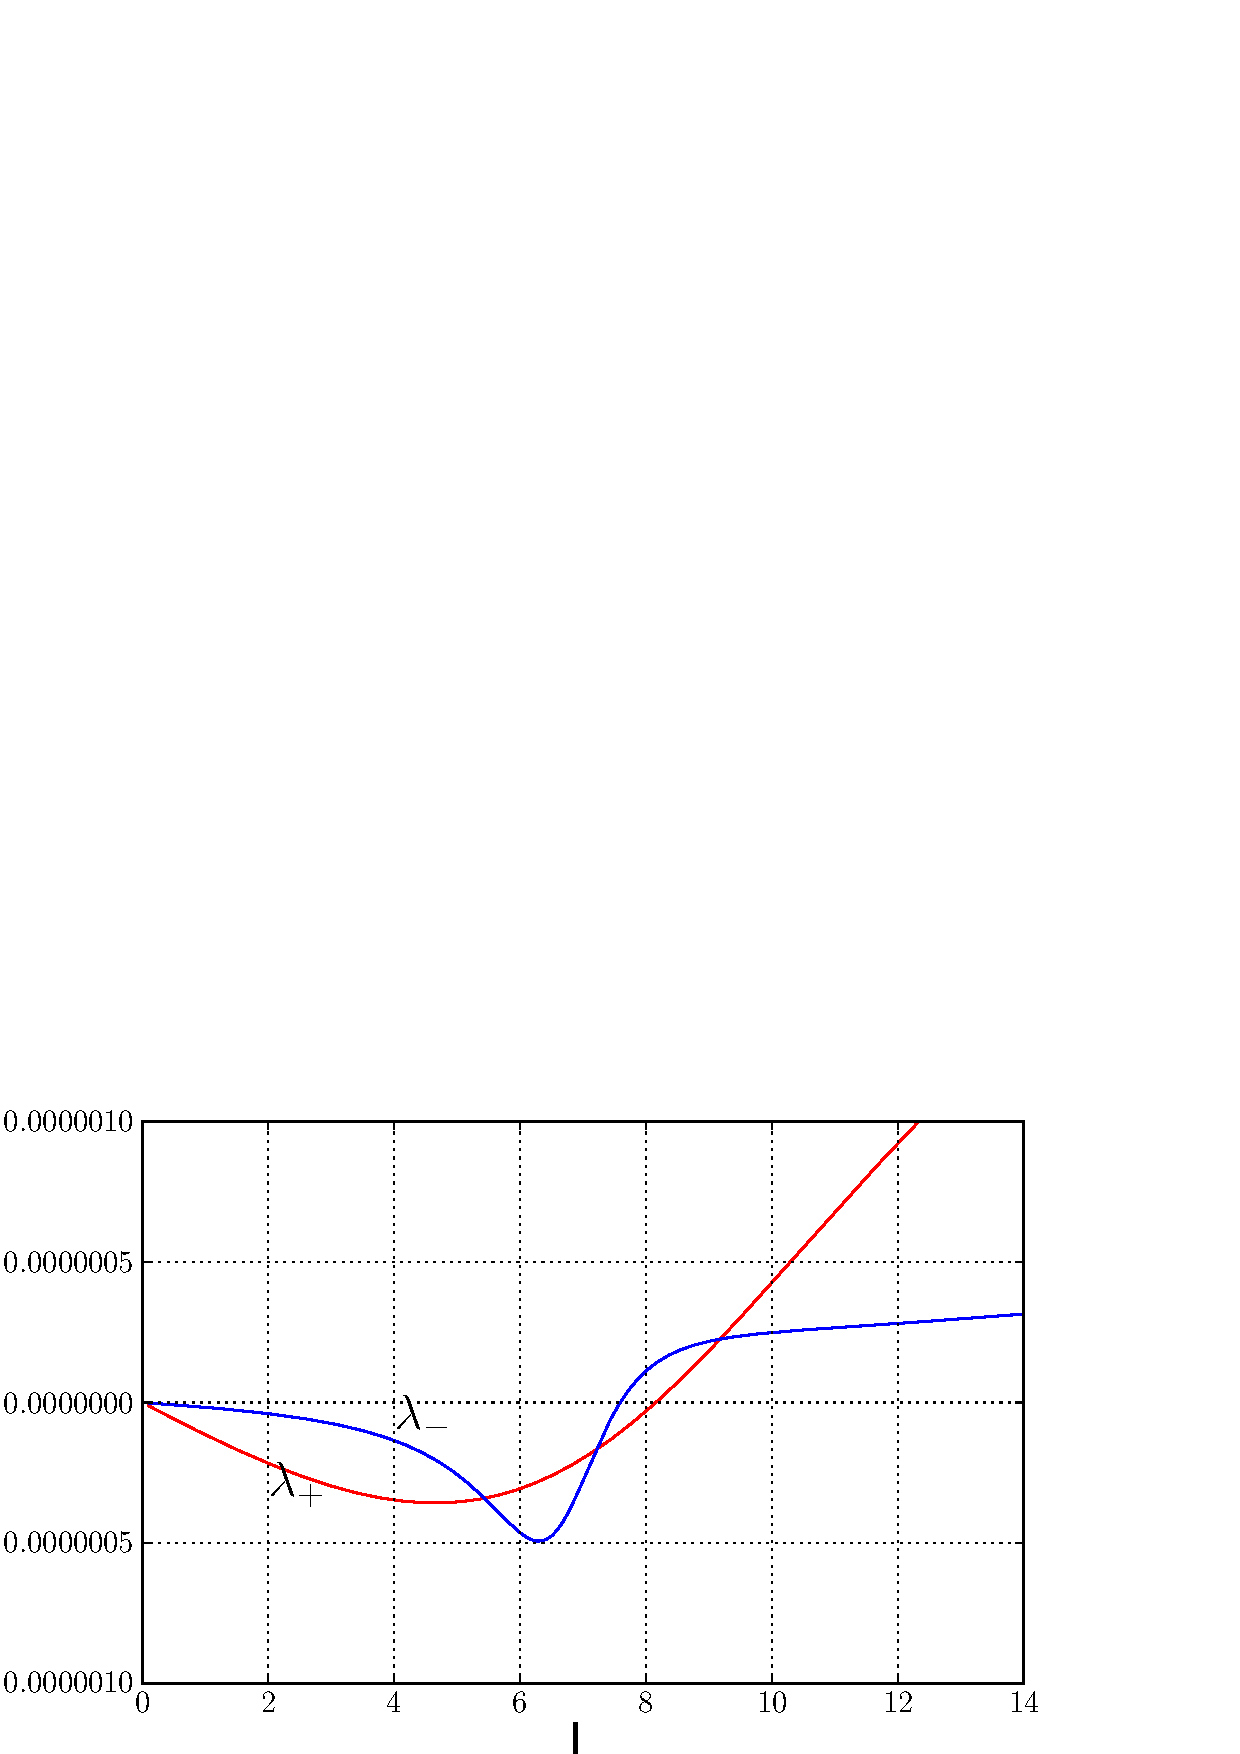
\includegraphics[height=1.5in]{lambda_L_kappa_1}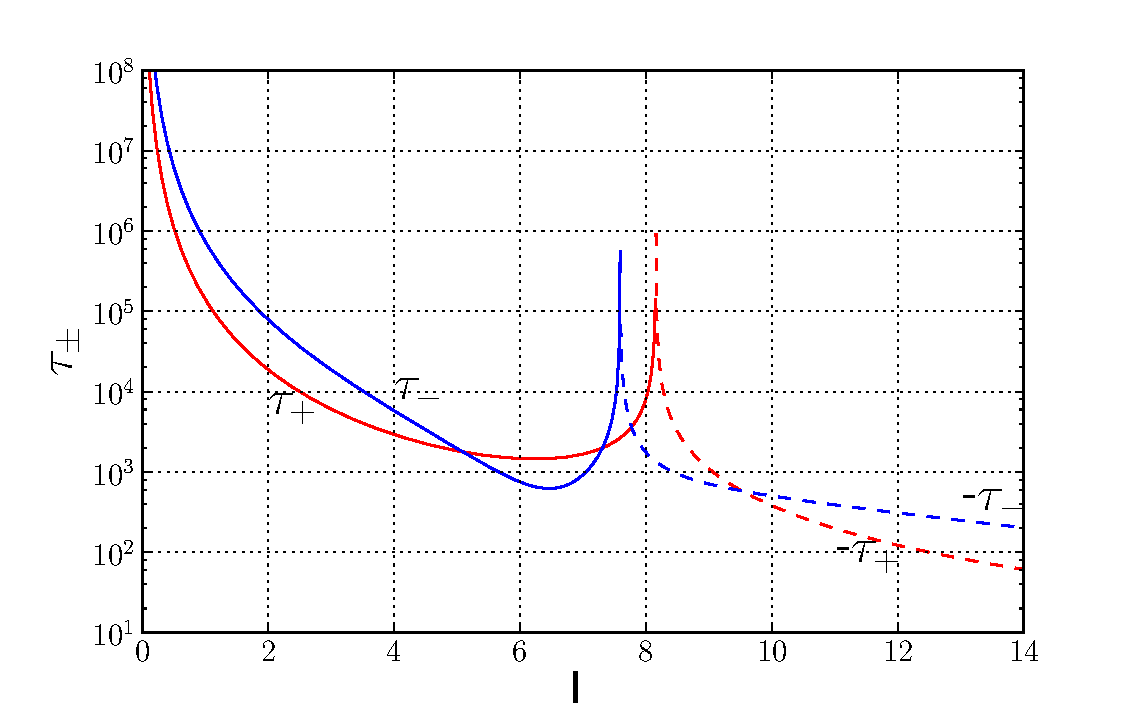
\includegraphics[height=1.5in]{tau_L_kappa_1}\\
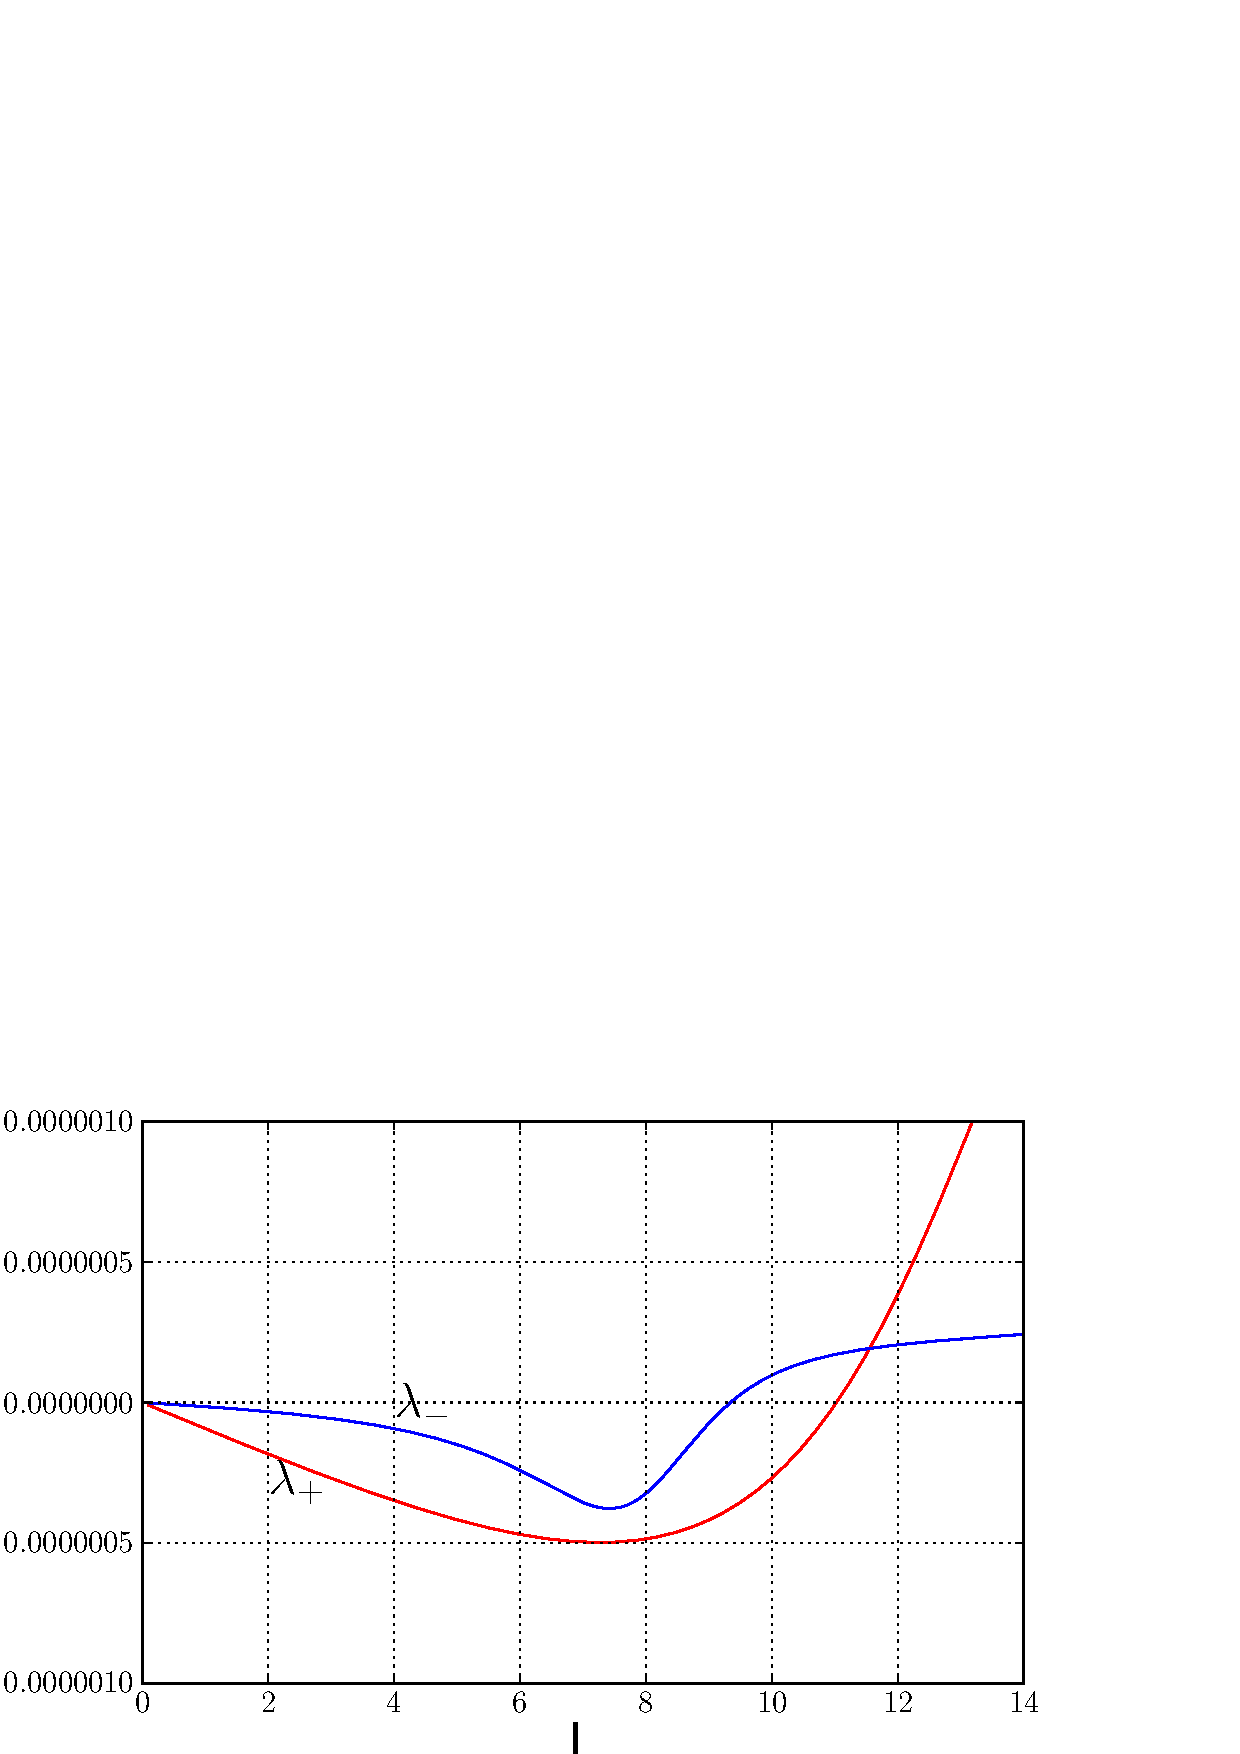
\includegraphics[height=1.5in]{lambda_L_kappa_065}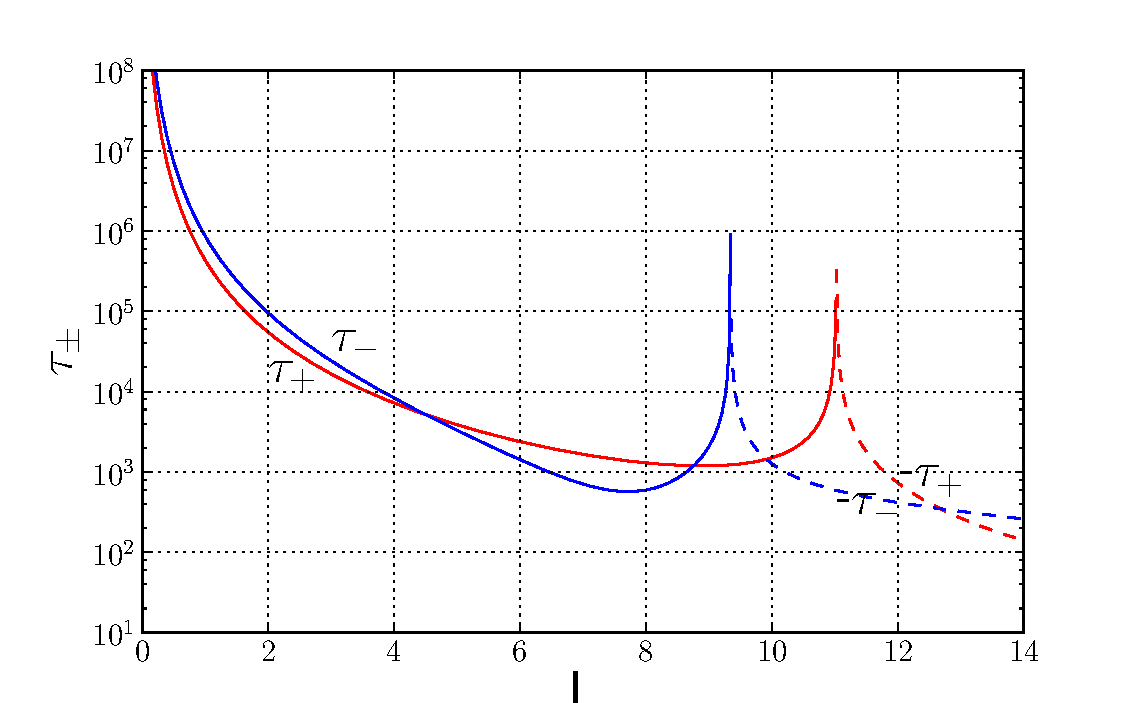
\includegraphics[height=1.5in]{tau_L_kappa_065}
\caption{Plots of both $\tau$ and $\lambda$ as a function of the domain length $L$. The parameters used in the computations are $D=50$, $\Ep=0.01$. The two top figures used $\kappa=1$, and the bottom figures $\kappa=0.65$.}
\label{fig:hopf1}
\end{center}
\end{figure}
% 

Using a straightforward Newton method the system can be easily solved, Figure \ref{fig:hopf1} shows the Hopf curves for both $\lA$ and $\tau$. At the point where the eigenvalues become positive, the critical value of $\tau$ becomes discontinuous, and throughout the range where $\lambda_{\pm}$ remains negative the breather eigenvalue is always smaller for small values of $L$, and in some cases the zigzag eigenvalue can become smaller. A similar thing happens with the critical $\tau$ values, although their behaviour doesn't exactly mimic the eigenvalues, as seen in the two bottom images in figure \ref{fig:hopf1}.
% 
\begin{figure}[htb]
\begin{center}
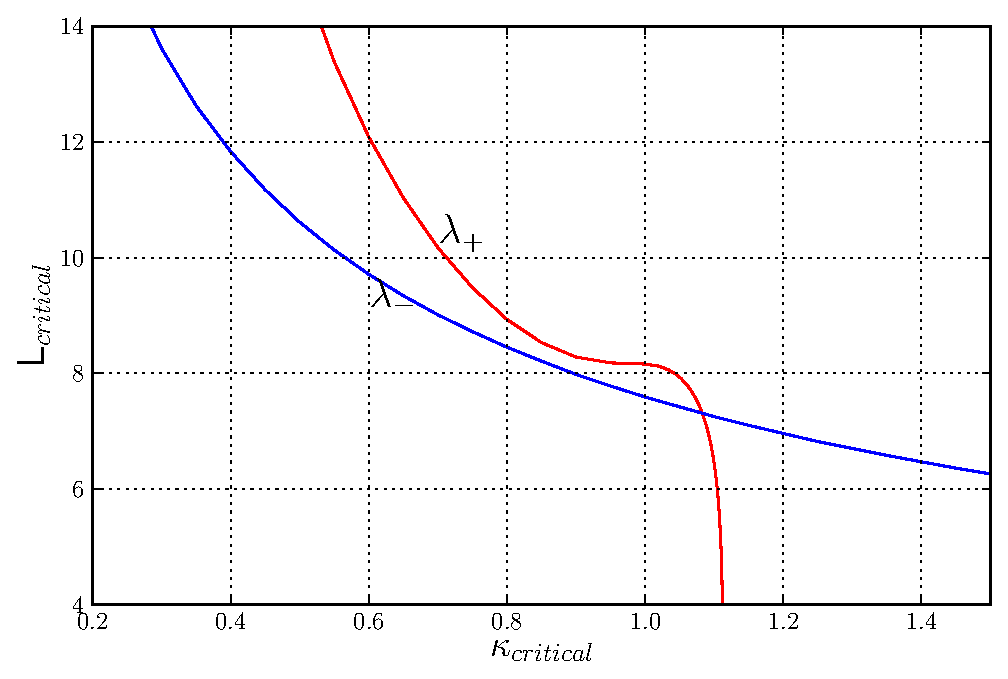
\includegraphics[height=2.5in]{kappa_hopf_critical_}
\caption{The critical values of $(\kappa,L)$ at which the breather and zigzag eigenvalues change sign.}
\label{fig:hopf_kappa}
\end{center}
\end{figure}
% 


We will now compute a full time-dependent solution for the case where $\tau=O(\Ep^{-3})$, and $\lA=O(\Ep^2)$.

We start again with the full system \eqref{eqn:gms1},
% 
\begin{equation*}
\label{eqn:gms2}
\begin{split}
\begin{aligned}
	u_t &= \Ep^2\De u + f(u,v) \\
	\tau v_t &= \frac{\DD}{\Ep}\De v + g(u,v),
\end{aligned}
\end{split}
\end{equation*}
% 
where we look for a time-dependent mesa solution (???figure) on the domain $[-L,L]$, with the two interfaces located at $x=l_1$ and $x=l_2$. Since $\lA=O(\Ep^2)$, the proper time scale the interfaces  is
% 
\[
  l_1 \equiv l_1(\Ep^2t);\qquad l_2 \equiv l_2(\Ep^2t).
\]
% 

We also let $\tau = \tilde{\tau}_0/\Ep^3$, and we define $T = \Ep^2t$.

We have then that \eqref{eqn:gms1} becomes
% 
\begin{equation}
\label{eqn:gms3}
\begin{split}
\begin{aligned}
	\Ep^2u_T &= \Ep^2\De u + f(u,v) \\
	\frac{\tilde{\tau}_0}{\Ep} v_t &= \frac{\DD}{\Ep}\De v + g(u,v).
\end{aligned}
\end{split}
\end{equation}
% 

We now do an asymptotic expansion near around the rightmost layer (a similar expansion will also have to be computed for the leftmost layer), with 
% 
\[
\begin{split}
  u &= U_0(y_1)+\Ep U_{1R}(y_1)+\cdots,\\
  v &= V_0 + \Ep V_{1R} + \Ep^2V_{2R} + \cdots,
\end{split}
\]
% 
where $y = \Ep^{-1}(x-l_1(T))$, and therefore $u_T = -\Ep^{-1}U_0'l_1'$. Substituting into \eqref{eqn:gms3}, we obtain that
% 
\[
  -\Ep^{-1}U_0'l_1' = U_0''+\Ep U_{1R}''+f(U_0,V_0) + \Ep f_U^0U_{1R} + \Ep f_V^0V_{1R}+\cdots
\]
% 

As before we take $V_0=$ constant, and define $u_+,u_-,V_0$ in terms of the Maxwell heteroclinic line condition
% 
\[
  \int_{u_-}^{u_+}f(u,V_0)du=0,\qquad f(u_{\pm},V_0)=0,\qquad f_u(u_{\pm},V_0)<0.
\]
% 

Thus, around the right transition layer we have
% 
\[
  U_{1R}''+f_u^0U_{1R} = -f_V^0V_{1R} - l_1'U_0',\qquad -\infty<x<\infty.
\]
% 

Similarly, for the $V$ equation we have
% 
\[
  \tilde{V}_0V_{1T} = \frac{\DD}{\Ep^3}(V_0'' + \Ep V_1''+\cdots) + g(U_0,V_0)+\cdots
\]
% 

Since $V_0=$ constant we have that 
% 
\[
  O(1) = \frac{1}{\Ep^2}\DD V_{1R}'' + O(1),
\]
% 
therefore $V_{1R}'' = 0$. We also have that $V\sim V_0$ on the entire interval, therefore in the internal region we cannot have $V_{1R}$ growing at infinity, hence
% 
\[
  V_{1R} = V_{1R}(T),
\]
% 
independent of $y$.

The inner problem on the rightmost layer is 
% 
\[
  \LL U_1 \equiv U_1'' + f_u^0 U_1 = -f_v^0 V_{1R} - l_1'U_0'.
\]
% 

Since $\LL U_0' = 0$, the solvability condition is
% 
\[
  -l_1'\int_{-\infty}^{\infty}U_0'^2dy - V_{1R}\int_{-\infty}^{\infty}f_v^0U_0'dy = 0,
\]
% 
and as we did before, since $U_0$ is a heteroclinic connection, 
% 
\[
  \int_{-\infty}^{\infty}f_v^0U_0'dy = \int_{u_+}^{u_-}f_v^0dU_0 = -\int_{u_-}^{u_+}f_v^0dU_0.
\]
% 

Thus, the ODE for the rightmost layer is
% 
\[
  l_1' = \frac{dl_1}{dT} = V_{1R}(T)\frac{\int_{u_-}^{u_+}f_v^0dU_0}{\int_{-\infty}^{\infty}U_0'^2dy}.
\]
% 

The same procedure on the leftmost layer at $x = l_2$ yields that
% 
\[
  l_2' = -V_{1L}(T)\frac{\int_{u_-}^{u_+}f_v^0dU_0}{\int_{-\infty}^{\infty}U_0'^2dy}.
\]
% 

To find values for $V_{1L}$ and $V_{1R}$ we need to match with the outer solution

